%% ----------------------------------------------------------------
%% Thesis.tex -- MAIN FILE (the one that you compile with LaTeX)
%% ----------------------------------------------------------------
% Set up the document
\documentclass[a4paper, 11pt, oneside]{Thesis}  % Use the "Thesis" style, based on the ECS Thesis style by Steve Gunn
\graphicspath{Figures/}  % Location of the graphics files (set up for graphics to be in PDF format)
% Include any extra LaTeX packages required
\usepackage{changepage}
\usepackage{fancyhdr}
\usepackage{float}
\usepackage{import}
\usepackage{lipsum}
\usepackage[square, numbers, comma, sort&compress]{natbib}  % Use the "Natbib" style for the references in the Bibliography
\usepackage{setspace}
\hypersetup{urlcolor=blue, colorlinks=true}  % Colours hyperlinks in blue, but this can be distracting if there are many links.
\usepackage{vector}  % Allows "\bvec{}" and "\buvec{}" for "blackboard" style bold vectors in maths
\usepackage{verbatim}  % Needed for the "comment" environment to make LaTeX comments
\usepackage{subfig}
\usepackage{graphicx}
\usepackage{gensymb}
\usepackage{afterpage, geometry, pdflscape, tabularx, ulem} % for landscape tables
\usepackage{multirow}
\usepackage{pdfpages}

\newgeometry{left=2in,right=0in,bottom=0in,top=2in}

% Use this to change the margin width for a snippet of text/table/figure etc.
\def\changemargin#1#2{\list{}{\rightmargin#2\leftmargin#1}\item[]}
\let\endchangemargin=\endlist

\def \thesistitle{Sensing and Actuation in Electroactive Elastomeric Bodies}
% Other thesis title ideas:
% Soft Electroactive Elastomeric Bodies that Can Sense and Contract
% Conductive Particle Elastomers as Artificial Skins and Actuators

%% ----------------------------------------------------------------
\begin{document}
	\frontmatter      % Begin Roman style (i, ii, iii, iv...) page numbering
	% Set up the Title Page
	\title  {\thesistitle}
	\authors  {\texorpdfstring
		{\href{ellingham.richie@gmail.com}{Richard James Morrin Ellingham}}
		{Richard James Morrin Ellingham}
	}
	\addresses  {\groupname\\\deptname\\\univname}  % Do not change this here, instead these must be set in the "Thesis.cls" file, please look through it instead
	\date       {\today}
	\subject    {}
	\keywords   {}
	\maketitle
	%% ----------------------------------------------------------------
	\setstretch{1.5}  % It is better to have smaller font and larger line spacing than the other way round
	% Define the page headers using the FancyHdr package and set up for one-sided printing
	\fancyhead{}  % Clears all page headers and footers
	\rhead{\thepage}  % Sets the right side header to show the page number
	\lhead{}  % Clears the left side page header
	\pagestyle{fancy}  % Finally, use the "fancy" page style to implement the FancyHdr headers
	%% ----------------------------------------------------------------
	% Declaration Page required for the Thesis, your institution may give you a different text to place here
	\Declaration{
		\addtocontents{toc}{\vspace{1em}}  % Add a gap in the Contents, for aesthetics
		I, AUTHOR NAME, declare that this thesis titled, `\thesistitle' and the work presented in it are my own. I confirm that:
		\begin{itemize}
			\item[\tiny{$\blacksquare$}] This work was done wholly or mainly while in candidature for a research degree at this University.
			\item[\tiny{$\blacksquare$}] Where any part of this thesis has previously been submitted for a degree or any other qualification at this University or any other institution, this has been clearly stated.
			\item[\tiny{$\blacksquare$}] Where I have consulted the published work of others, this is always clearly attributed.
			\item[\tiny{$\blacksquare$}] Where I have quoted from the work of others, the source is always given. With the exception of such quotations, this thesis is entirely my own work.
			\item[\tiny{$\blacksquare$}] I have acknowledged all main sources of help.
			\item[\tiny{$\blacksquare$}] Where the thesis is based on work done by myself jointly with others, I have made clear exactly what was done by others and what I have contributed myself.
			\\
		\end{itemize}
		Signed:\\
		\rule[1em]{25em}{0.5pt}  % This prints a line for the signature
		Date:\\
		\rule[1em]{25em}{0.5pt}  % This prints a line to write the date
	}
	\clearpage  % Declaration ended, now start a new page
	%% ----------------------------------------------------------------
	% The "Funny Quote Page"
	\pagestyle{empty}  % No headers or footers for the following pages
	\null\vfill
	% Now comes the "Funny Quote", written in italics
	\textit{``When do you think you can submit your thesis?''}
	\begin{flushright}
		T. Giffney, April 2024
	\end{flushright}
	\textit{``Today.''}
	\begin{flushright}
		R. Ellingham, September 2024
	\end{flushright}
	\vfill\vfill\vfill\vfill\vfill\vfill\null
	\clearpage  % Funny Quote page ended, start a new page
	\setstretch{1.5}
	%% ----------------------------------------------------------------
	% The Abstract Page
	\addtotoc{Abstract}  % Add the "Abstract" page entry to the Contents
	\abstract{\addtocontents{toc}{\vspace{1em}}  % Add a gap in the Contents, for aesthetics
		% 
		Some of the world's most advanced technology is rigid due to various factors such as; manufacturability, miniaturisability, physical linearity, and more ideal physics in general. In parallel industries is also looking to use automation to improve and replace laborious tasks whether they be domestic, commercial, or industrially related tasks. Their is a growing need for new innovations in technology to utilise the soft robotic solutions that mimic biological solutions seen in nature. This thesis is part of many to improve an understanding of the electroactive polymer subset of soft robotics and the limitations of specific implementations of artificial skin and artificial muscle technologies.
		
		This thesis explores the integration of Electrical Impedance Tomography (EIT) with advanced soft sensing technologies, focusing on carbon black silicone rubber (CBSR) elastomer composites and Dielectric Elastomer Actuators (DEAs) to enhance pressure mapping, strain sensing, and actuation.
		
		CBSR elastomer composites, noted for their high stretchability and biocompatibility, were investigated to understand their resistance relaxation behavior. This research contributes to optimizing the design of flexible dynamic strain sensors by modeling the response of resistance to transient strain inputs. The study developed an EIT-based pressure mapping system using a silicone CB nanoparticle sensing domain that mimics pressure mapping qualities human skin. This system was evaluated for its spatial and temporal resolution, showing potential for creating artificial pressure-sensitive skin with practical applications. Furthermore, the integration of EIT with DEAs was examined to improve the mapping of compressive forces across electrode surfaces. Despite some trade-offs in accuracy due to electrode compliance, this approach offers promising advancements for applications requiring precise actuation and pressure mapping. This work has majorly contributed towards filing a patent for an DEA-EIT actuator-sensor device. Additionally, the research uncovered unintentional power generation in DEAs, which could function as Dielectric Elastomer Generators (DEGs) due to mechanical strain. This finding highlights the dual functionality of DEAs and suggests opportunities for energy harvesting applications. Finally, a portable, low-cost EIT-based hardware system for pressure mapping was introduced. This system enables comprehensive characterization of various sensing domains and supports advancements in EIT-based soft sensor technology, with implications for biomedical devices, robotics, and energy harvesting. 
		
		Overall, this research advances the field of soft sensors by integrating EIT with innovative materials and technologies, providing new insights and applications in dynamic sensing and actuation.
	}
	\clearpage  % Abstract ended, start a new page
	%% ----------------------------------------------------------------
	\setstretch{1.3}  % Reset the line-spacing to 1.3 for body text (if it has changed)
	% The Acknowledgements page, for thanking everyone
	\acknowledgements{
		\addtocontents{toc}{\vspace{1em}}  % Add a gap in the Contents, for aesthetics
		People to thank:
		\begin{itemize}
			\item UC Bioengineering office - Lung lads, Lung Ladies, IPC, Hamish for infinite beers, Nic's abstract art.
			\item Geoff Chase - for a constant stream of stories and advice always within earshot.
			\item Other office - for ping pong madness, bikkies and fruit.
			\item Supervisor Tim - for time, money, lack of time, and support on a project that slightly diverged from his research till the end.
			\item Co-supervisors Chris, and late comer Lui - for advice and casual yarns.
			\item Summer students Toby and Yeni - for great work towards my PhD topic.
			\item UC mechanical and electrical department technicians (Julian Murphy, Julian Phillips, Tony Doyle, Scott Lloyd, amongst others) - for general support and yarns throughout my maddness.
			\item Juan Jose and Anastasia at IMDEA Materiales - for help with me going down a wonderful materials science rabbit hole.
			\item Markus Vorrath and co. at TU Dresden - for giving me a home to type out words and a group to discuss soft robotics with.
			\item Johannes Mersch - For helping with some final (hopefully groundbreaking) experiments when I was in strife towards the end of my PhD.
			\item Tess - for general oddities, support, and love.
			\item Friends - for constantly questioning "so when are you finishing again?"
			\item Family - for being supportive.
		\end{itemize}
	}
	\clearpage  % End of the Acknowledgements
	%% ----------------------------------------------------------------
	\pagestyle{fancy}  %The page style headers have been "empty" all this time, now use the "fancy" headers as defined before to bring them back
	%% ----------------------------------------------------------------
	\lhead{\emph{Contents}}  % Set the left side page header to "Contents"
	\tableofcontents  % Write out the Table of Contents
	%% ----------------------------------------------------------------
	\lhead{\emph{List of Figures}}  % Set the left side page header to "List if Figures"
	\listoffigures  % Write out the List of Figures
	%% ----------------------------------------------------------------
	\lhead{\emph{List of Tables}}  % Set the left side page header to "List of Tables"
	\listoftables  % Write out the List of Tables
	%% ----------------------------------------------------------------
	\setstretch{1.5}  % Set the line spacing to 1.5, this makes the following tables easier to read
	\clearpage  % Start a new page
	\lhead{\emph{Abbreviations}}  % Set the left side page header to "Abbreviations"
	\vspace{-0.5cm}
	\listofsymbols{ll}  % Include a list of Abbreviations (a table of two columns)
	{
		% \textbf{Acronym} & \textbf{W}hat (it) \textbf{S}tands \textbf{F}or \\
		\textbf{ADC} & \textbf{A}nalog-\textbf{t}o-\textbf{D}igital \textbf{C}onverter \\
		\textbf{CAD} & \textbf{C}omputer \textbf{A}ided \textbf{D}esign \\
		\textbf{CB} & \textbf{C}arbon \textbf{B}lack \\
		\textbf{CFA} & \textbf{C}artesian \textbf{F}orce \textbf{A}pplicator \\
		\textbf{CE} & \textbf{C}ompliant \textbf{E}electrode \\
		\textbf{CoM} & \textbf{C}enter of \textbf{M}ass \\
		\textbf{DE} & \textbf{D}ielectric \textbf{E}lastomer \\
		\textbf{DEA} & \textbf{D}ielectric \textbf{E}lastomer \textbf{A}ctuator \\
		\textbf{DEG} & \textbf{D}ielectric \textbf{E}lastomer \textbf{G}enerator \\
		\textbf{DUT} & \textbf{D}omain \textbf{U}nder \textbf{T}est \\
		\textbf{EIT} & \textbf{E}lectrical \textbf{I}mpedance \textbf{T}omography \\
		\textbf{ERT} & \textbf{E}lectrical \textbf{R}esistance \textbf{T}omography \\
		\textbf{FEA} & \textbf{F}inite \textbf{E}lement \textbf{A}nalysis \\
		\textbf{FEM} & \textbf{F}inite \textbf{E}lement \textbf{M}odelling \\
		\textbf{FPC} & \textbf{F}lexible \textbf{P}rinted \textbf{C}ircuit \\
		\textbf{IDF} & \textbf{I}oT \textbf{D}evelopment \textbf{F}ramework \\
		\textbf{MUX} & \textbf{M}ultiplexer \\
		\textbf{PCB} & \textbf{P}rinted \textbf{C}ircuit \textbf{B}oard \\
		\textbf{PCBA} & \textbf{P}rinted \textbf{C}ircuit \textbf{B}oard \textbf{A}ssembly\\
		\textbf{PDMS} & \textbf{P}oly\textbf{d}i\textbf{m}ethyl\textbf{s}iloxane (AKA silicone)\\
		\textbf{PNEC} & \textbf{P}iezoresistive \textbf{N}anoparticle \textbf{E}lastomer \textbf{C}omposite\\
		\textbf{SMU} & \textbf{S}ource \textbf{M}easure \textbf{U}nit \\
		\textbf{SMD} & \textbf{S}urface-\textbf{M}ount \textbf{D}evice \\
		\textbf{SR} & \textbf{S}ilicone \textbf{R}ubber \\
		\textbf{THT} & \textbf{T}hrough-\textbf{H}ole \textbf{T}echnology \\
		\textbf{EAP} & \textbf{E}lectro-\textbf{A}ctive \textbf{P}olymer\\

	}
	%% ----------------------------------------------------------------
	
	\clearpage  %Start a new page
	\lhead{\emph{Nomenclature}}  % Set the left side page header to "Symbols"
	\listofnomenclature{lll}  % Include a list of Symbols (a three column table)
	{
		% symbol & name & unit \\
		$A$ & Area & [m$^2$] \\
		$C$ & Capacitance & [F] \\
		$\epsilon_0$ & Vacuum Permittivity & [Fm$^{-1}$] \\
		$\epsilon_r$ & Relative Permittivity & [a.u.] \\
		$K$ & Bulk Modulus & [Pa] \\
		$\nu$ & Poisson’s Ratio & [a.u.] \\
		$Q$ & Electrical Charge & [C] \\
		$U_E$ & Electrical Potential Energy & [J] \\
		$U_{\epsilon}$ & Elastic Potential Energy & [J] \\
		$R$ & Resistance & [$\Omega$] \\
		$\sigma$ & Stress & [Pa] \\
		$S$ or $\varepsilon$ & Strain & [a.u. or \%] \\ % change this to S or \varepsilon?
		$\dot\varepsilon$ & Strain Rate & [\%s$^{-1}$] \\
		$V$ & Voltage & [V] \\
		$Y$ or $E$ & Young's Modulus & [Pa] \\
		$z$ & Thickness & [m] \\

		
	}
	%% ----------------------------------------------------------------
	% End of the pre-able, contents and lists of things
	% Begin the Dedication page
	\setstretch{1.0}  % Return the line spacing back
	\pagestyle{empty}  % Page style needs to be empty for this page
	\dedicatory{Dedicated to tinned baked beans in all their glory\ldots}
	\addtocontents{toc}{\vspace{2em}}  % Add a gap in the Contents, for aesthetics
	%% ----------------------------------------------------------------
	\mainmatter	  % Begin normal, numeric (1,2,3...) page numbering
	\pagestyle{fancy}  % Return the page headers back to the "fancy" style
	% Include the chapters of the thesis, as separate files
	% Just uncomment the lines as you write the chapters
	\lhead{\emph{\chapiname}}
	\import{Chapters/}{Chapter1.tex} % Introduction
	\lhead{\emph{\chapiiname}}
	\import{Chapters/}{Chapter2.tex} % Literature Review
	\lhead{\emph{\chapiiiname}}
	\import{Chapters/}{Chapter3.tex} % CBSR behaviour
%	\lhead{\emph{\chapivname}}
%	\import{Chapters/}{Chapter4.tex} % Improved EIT-based sensor
%	\lhead{\emph{\chapvname}}
%	\import{Chapters/}{Chapter5.tex} % DEA-EIT 
%	\lhead{\emph{\chapviname}}
%	\import{Chapters/}{Chapter6.tex} % DEA-EIT an unintended DEG
%	\lhead{\emph{\chapviiname}}
%	\import{Chapters/}{Chapter7.tex} % DEA-EIT hardware
%	\lhead{\emph{\chapviiiname}}
%	\import{Chapters/}{Chapter8.tex} % DEA-EIT capacitive modelling??
%	\lhead{\emph{\chapixname}}
%	\import{Chapters/}{Chapter9.tex} % Discussion and Conclusion

	%% ----------------------------------------------------------------
	% Now begin the Appendices, including them as separate files
	\addtocontents{toc}{\vspace{2em}} % Add a gap in the Contents, for aesthetics
	\appendix % Cue to tell LaTeX that the following 'chapters' are Appendices
%	\chapter{Thesis Crossword}
\label{appendix-A}
\vspace{-2cm}
\begin{table}[H]
	\centering
	\begin{tabular}{p{\linewidth}}
		\hspace{1cm}
		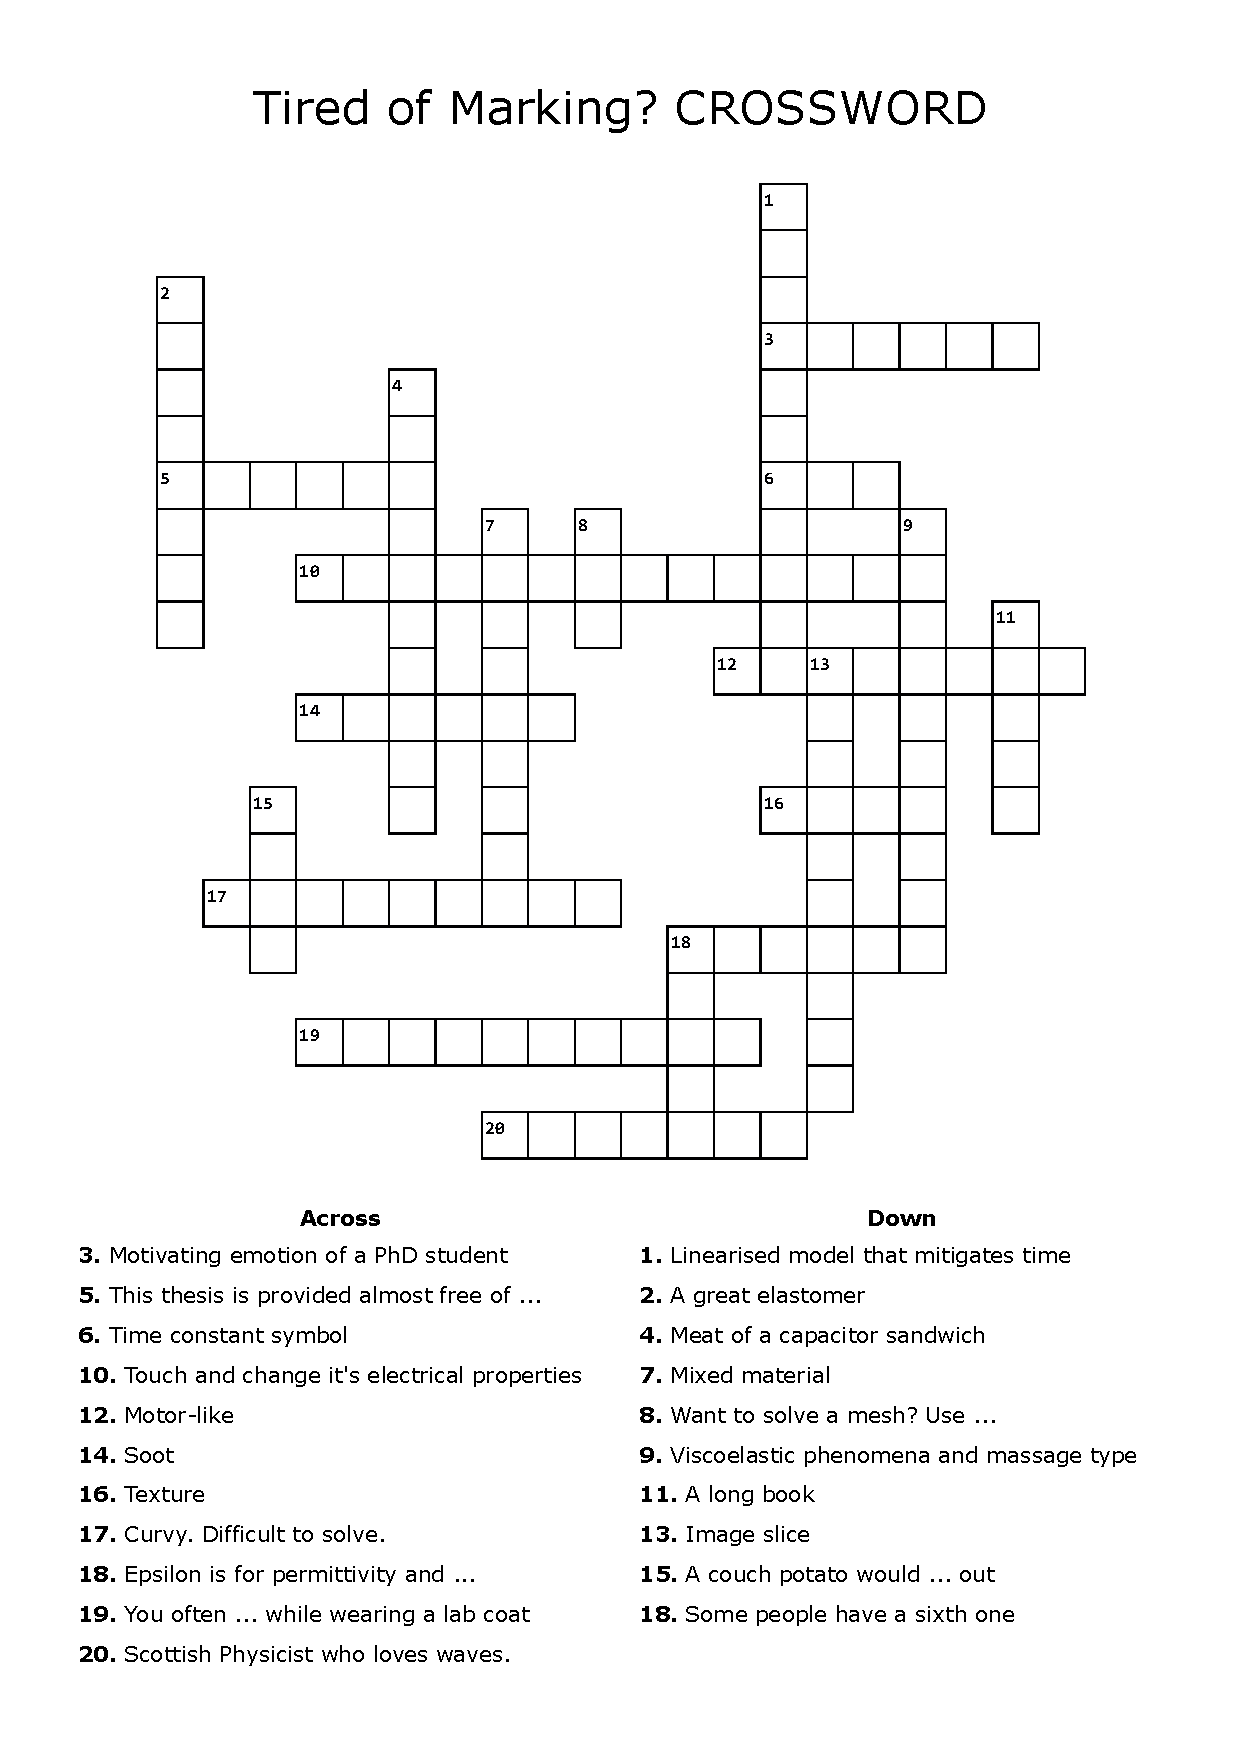
\includegraphics[width=0.85\linewidth]{fun-thesis-crossword.pdf}
	\end{tabular}
\end{table}
%\includepdf[pages=-,scale=0.2,offset=70 0]{}
	% Appendix Title
	%\chapter{Strain-Stress-Resistance Experiments}
\label{appendix-B}
%\section{title}
\begin{figure}[H]
	\centering
	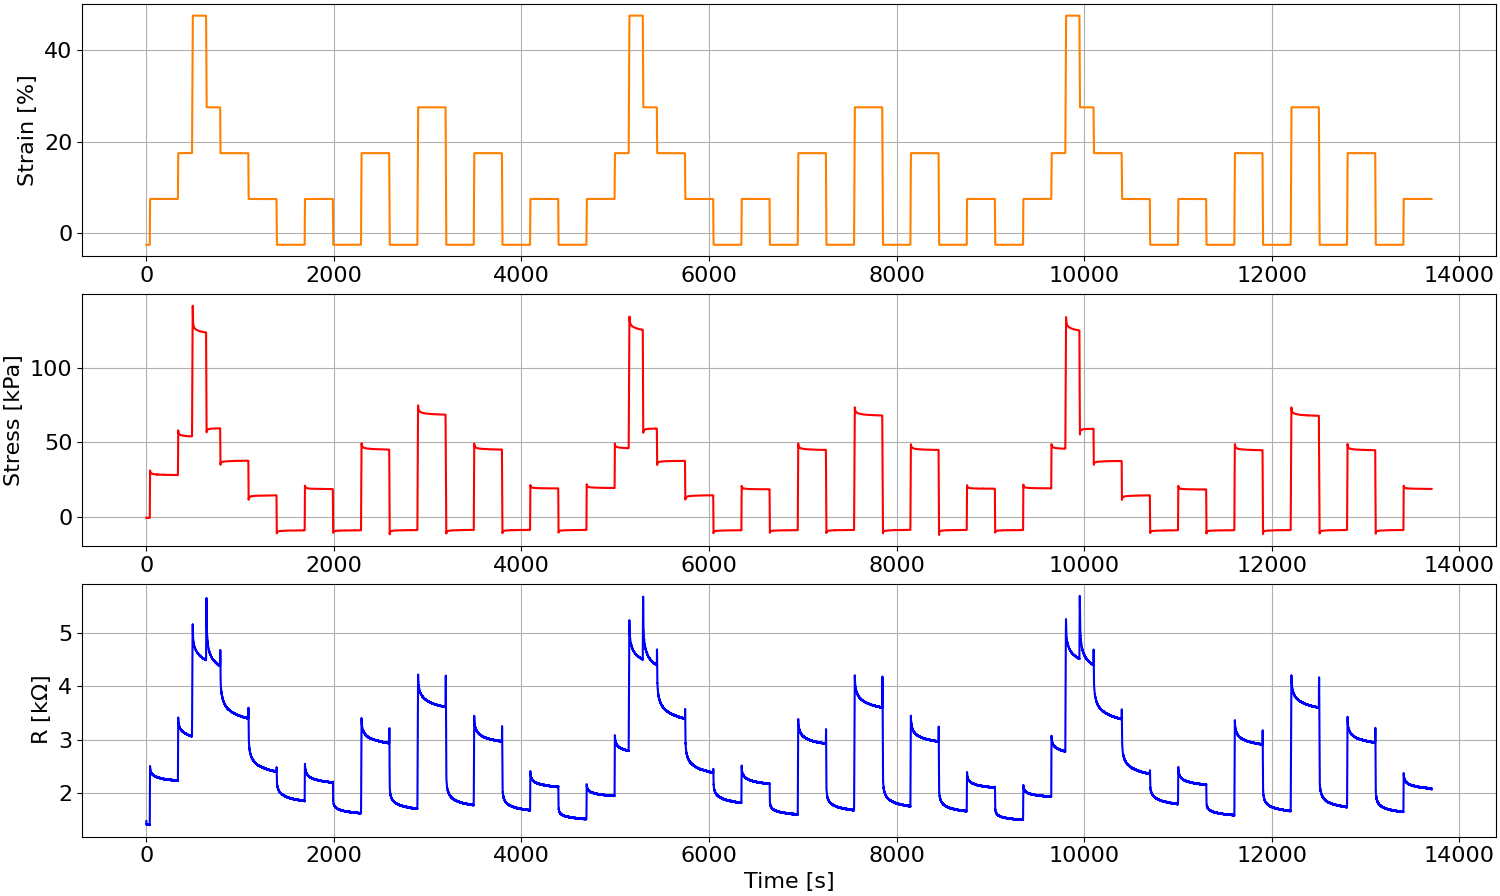
\includegraphics[width=\linewidth]{Figures/2_7-5_E4pin_20mm_v12_0.1_0.2_0.3_strain_1mm_offset_erroneous.png}
	\caption{Strain test sequence showing the shoulder phenomena correlation for varying magnitudes of strain for a 7.5 wt\% CBSR specimen dogbone sample. This experiment had an unintentional offset of 1 mm, however this showed a drastic decrease shoulder phenomena when the falling edge is crossing the x-axis.}
	\label{fig:strain-hill}
\end{figure}
\begin{figure}[H]
	\centering
	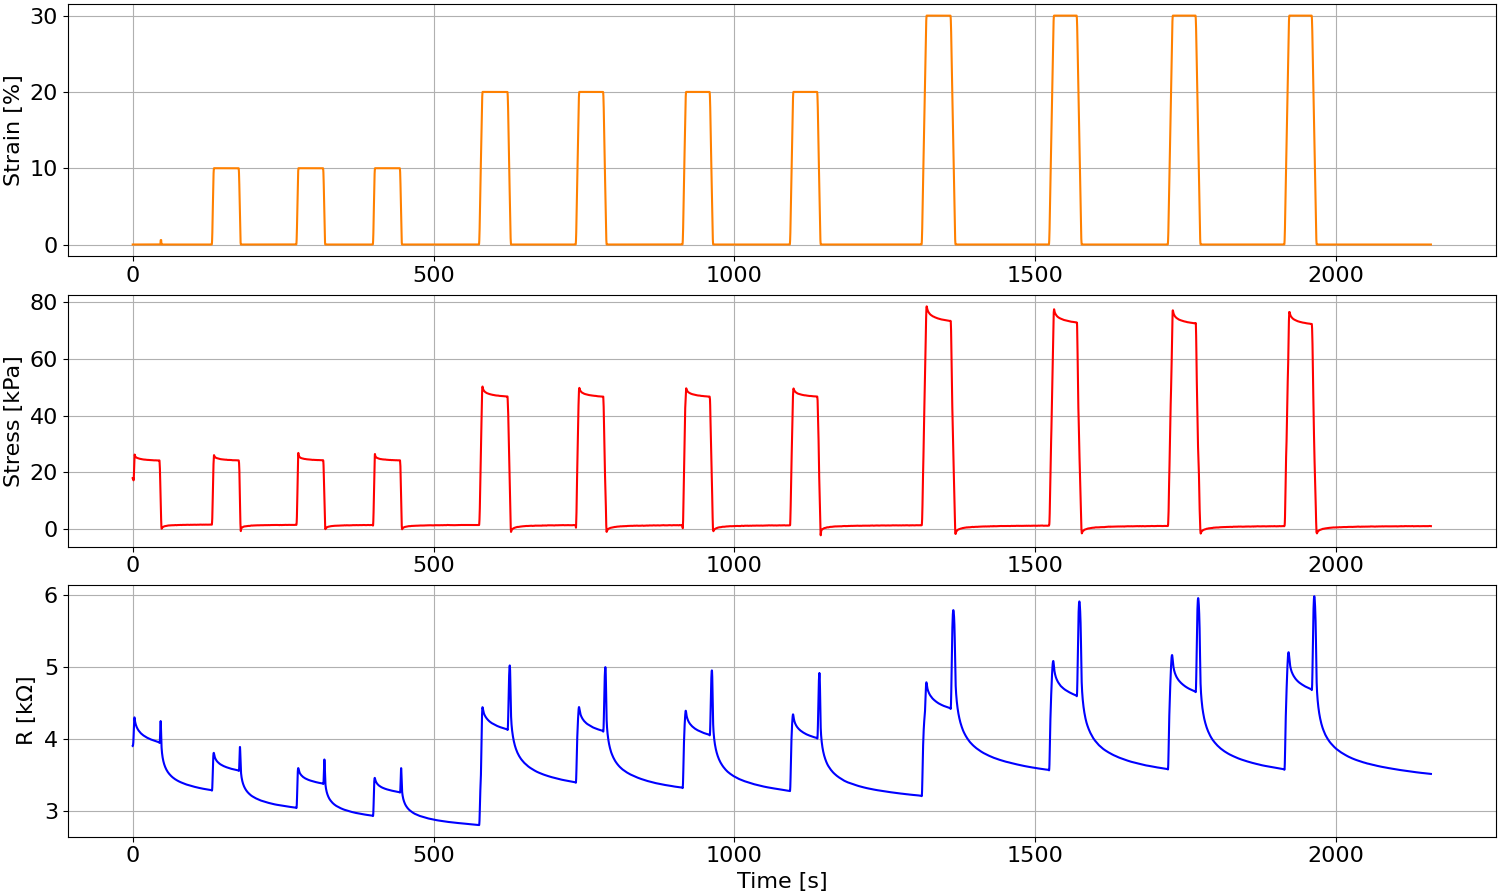
\includegraphics[width=\linewidth]{Figures/1_7-5_Epin_20mm_v2_DC_meas_3_strains.png}
	\caption{Strain test sequence showing the shoulder phenomena correlation for varying magnitudes of strain for a 7.5 wt\% CBSR specimen dogbone sample. This experiment used DC measurements, so the macro downward trend in resistance is more obvious than other experimental data given in this work with used a switched AC signal.}
	\label{fig:strain-train-DC-meas}
\end{figure}
\begin{figure}[H]
	\centering
	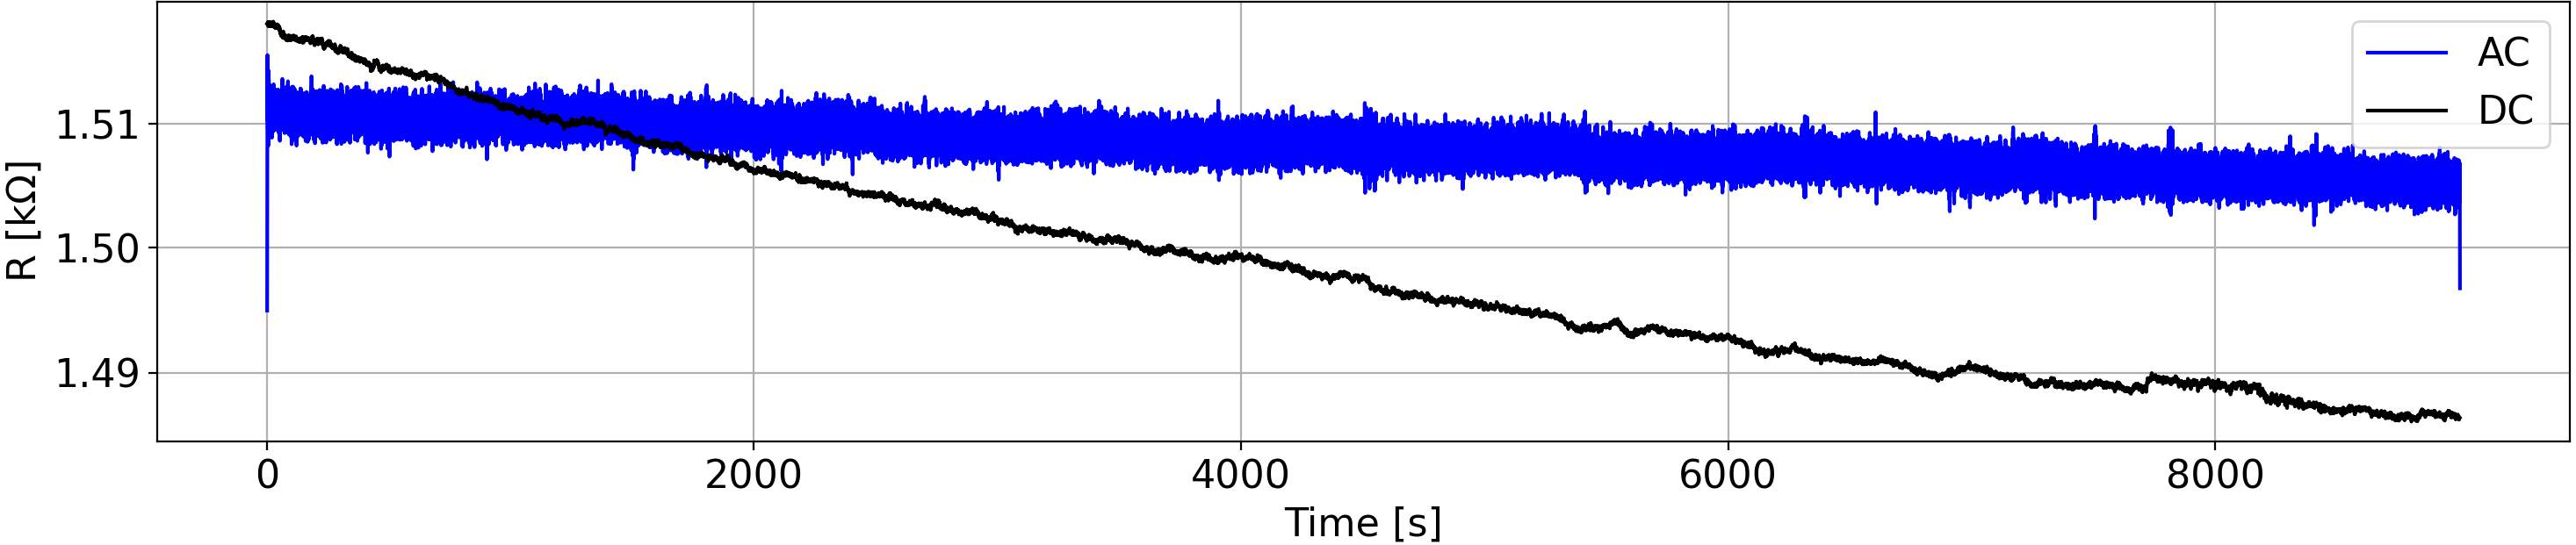
\includegraphics[width=\linewidth]{Figures/AC_vs_DC_long_decay_2_7-5_CBSR}
	\caption{AC vs DC downward trend in resistance for an unstrained 7.5 wt\% CBSR composite dogbone specimen.}
	\label{fig:res-AC-DC}
\end{figure}

 % Appendix Title
	%\chapter{Chapter Title}
\label{appendix-C}
 % Appendix Title
	\addtocontents{toc}{\vspace{2em}}  % Add a gap in the Contents, for aesthetics
	\backmatter
	%% ----------------------------------------------------------------
	\label{Bibliography}
	\lhead{\emph{Bibliography}}  % Change the left side page header to "Bibliography"
	\bibliographystyle{unsrtnat}  % Use the "unsrtnat" BibTeX style for formatting the Bibliography
	\bibliography{Bibliography}  % The references (bibliography) information are stored in the file named "Bibliography.bib"
\end{document}  % The End
%% ----------------------------------------------------------------